%\documentclass[a4paper]{article}
%\usepackage[utf8]{inputenc}
%\usepackage{amsthm}             % Definitions and such
%\usepackage{amssymb}            % R for space and such
%\usepackage{amsmath}
%\usepackage[a4paper]{geometry}
%
%\title{LINMA2471 : Optimization models and models : course 2 (23/09/2015)}
%\author{Antoine de Comité , Florimond Houssiau \& Vincent Schellekens}
%\date{September 2015}
%
%\usepackage{natbib}
%\usepackage{graphicx}
%\usepackage{framed}
%\usepackage{tikz}
%\usepackage{float}
%\usetikzlibrary{arrows}
%\usetikzlibrary{decorations.markings}
%
%
%\begin{document}
%
%
%
%\maketitle

In this chapter we will see some important classes of optimization problems, and some techniques to re-write an optimization problem into another form.

\section{Definitions and motivation}
First of all, let's recall what the model of an optimization problem looks like.\\

\begin{definition}
A \textbf{general model} has the following form :
\begin{equation}
\min_{x \in X \subseteq \mathbb{R}^n} f(x)
\end{equation}
where $x$ are the \textbf{variables}, X is the \textbf{feasible set} (also called domain or feasible region) and f is the \textbf{objective function}.
\end{definition}

Note that the feasible set $X$ is a subset of a \textit{finite} dimensional space. Optimization within infinite-dimensional spaces are not covered in this course.\\

Let us next introduce two very important classes of models : the \textit{linear} and \textit{convex} models.\\

\begin{definition}
A model is called a \textbf{linear model} if :
\begin{enumerate}
  \item The objective function is linear/affine\footnote{Note that the independent term of an affine function ($d$) can be easily dropped out, because it doesn't affect the optimal solution in any way. Therefore, every affine function can be replaced with a purely linear one.}, that is, of the form $c^T x/c^T x +d$.
  \item The feasible set X is a \textbf{polyhedron}. A polyhedron is an intersection of a finite\footnote{For example, a sphere is therefore \textit{not} a polyhedron, because it is an intersection of an \textit{infinite} number of closed half-planes.} number of closed \textbf{half-spaces}. As a reminder, a half-space is the set of points that lie on one side of a hyperplane; in an algebraïc form : $\{x \in \mathbb{R}^n | a^T x \geq b\}$ or $\{x \in \mathbb{R}^n | a^T x \leq b\}$.
\end{enumerate}
\end{definition}

\vspace{\baselineskip}
		
\begin{definition}
A model is called a \textbf{convex model} if :
\begin{enumerate}
  \item The objective function f is convex (see below). 
  \item The feasible set X is convex (see below).
\end{enumerate}
\end{definition}

We still need to define what are convex functions and sets :\\

\begin{definition}
    A set X is a \textbf{convex set} if it contains the segments between every pair of its points.
\end{definition}

\vspace{\baselineskip}

\begin{definition}
    A function f is a \textbf{convex function} if its \textbf{epigraph} is convex. The epigraph\footnote{Note that if $f : \mathbb{R}^n \to \mathbb{R}$ then $epi \: f \subseteq \mathbb{R}^{n+1}$} of f is the set of points above (and including) the graph of f. Formally, we write this as : $epi \: f := \{(x,t)|t \geq f(x)\} $. This notion is illustrated on Figure \ref{epi}.
\end{definition}

For the definition of convex functions, we didn't used the concept of derivative, because we want our definition to be as general as possible. In other words, a non-differentiable function can be convex\footnote{For example, the norm function defined by $f:\mathbb{R} \to \mathbb{R}: x \to |x|$ is convex}. Note also that \textit{every linear model is a particular case of a convex model}.\\


\begin{figure}[h!]
\centering
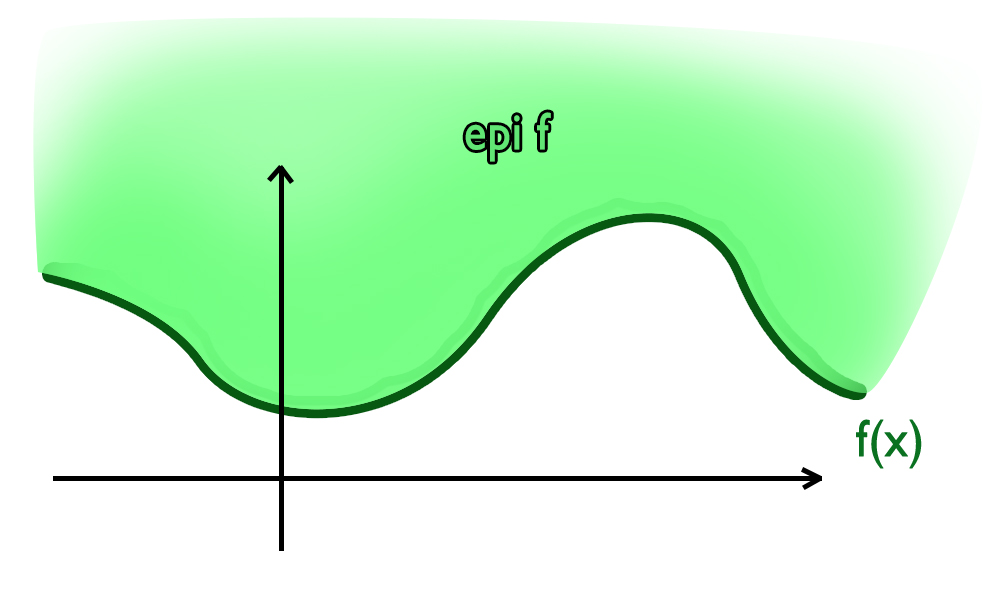
\includegraphics[scale=0.3]{./images/Course2_epi}
\caption{Illustration of the epigraph of some one-dimensional (and non-convex) function. The epigraph of $f$ is the region above the graph of $f$. }
\label{epi}
\end{figure}

Now that we know the definitions of linear and convex models, what is the \textbf{motivation} to study such models? First, these models are useful to develop \textit{efficient algorithms} with \textit{guarantees} about the exactitude of the optimal solution and the speed of the algorithm.

Also, one could argue that studying linear/convex models is a restriction to the number of problems we will be able to solve, but it turns out that convex problems are \textit{not so rare} in practice. Many problems are, or can be formulated as convex problems. Some problems can even be solved by using an equivalent convex problem : for example, the \textit{branch and bound} algorithm transforms a discrete (and therefore non-convex) problem into a sequence of linear problems. One last -informal- reason to restrict ourselves to convex problem is that, for non-convex problems, there is nothing interesting we can really do or say.


\section{Standard forms}
As the general formulation of convex and linear problems can be very hard to use in order to develop a theory about them, due (mostly) to the variety of constraint types, it is important to define \textbf{standard forms}. Standard forms define a unique, specific, formulation of these problems, that is much simpler than the general form.

\subsection{Linear case: re-writing objective function, variables and constraints}
Before we define the standard form, let us observe a number of transformations that can be applied to a linear problem without changing its solution (that is, the two problems will be equivalent).

\paragraph{Maximization and minimization}
In general, a maximization problem can easily be formulated as a minimization problem. Indeed, maximizing a function $f$ is equivalent to minimizing its opposite $-f$. If the solution $x$ is the same, the value of the objective function $-f(x)$ is simply the opposite of that of the original problem.

\begin{center}
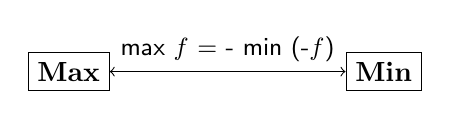
\begin{tikzpicture}[<->,node distance=4cm, main node/.style={rectangle,draw,font=\bfseries}]

  \node[main node] (1) {Max};
  \node[main node] (2) [right of=1] {Min};

  \path[every node/.style={font=\sffamily\small}]
    (1) edge node [above] {max $f$ = - min (-$f$)} (2);
\end{tikzpicture}
\end{center}

\paragraph{Non-negative variables}
The variables used in the linear standard form are non-negative, that is, they are free with the implicit constraint $x \geq 0$. It is possible to transform free variables in non-negative variables by a process known as \textbf{splitting}.

\begin{center}
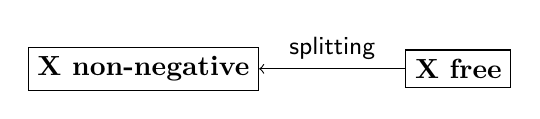
\begin{tikzpicture}[<-,node distance=4cm, main node/.style={rectangle,draw,font=\bfseries}]

  \node[main node] (1) {X non-negative};
  \node[main node] (2) [right of=1] {X free};

  \path[every node/.style={font=\sffamily\small}]
    (1) edge node [above] {splitting} (2);
\end{tikzpicture}
\end{center}

Splitting is done by, for every free variable $x_i$, adding two non-negative variables $x_i^+$ and $x_i^-$, defined by the relationship $x_i = x_i^+ - x_i^-$. Then, $x_i$ is substitued by $ x_i^+ - x_i^-$ everywhere in the problem.

However, this can be severely inefficient, since it adds a variable for every free variable. In a problem with $n$ free variables, $n$ additionnal variables are created, thus doubling the size of the problem. As this can be a major performance issue, it is important to do the splitting without creating too many variables. 

A simple observation about the current method that can be made is that, if we assume $x_i$ has a unique value in the solution, the values of $x_i^+$ and $x_i^-$ are not uniquely defined (in some sense, there is one too many degree of freedom). By exploiting this notion, another formulation can be proposed: if a problem has $n$ free variables $x_i$, we subtitute these by $x_i^+ - x^-$, where $x_i^+$ and $x^-$ are non-negative variable, and $x^-$ is \textbf{the same for all the variables}. This method is better since it only creates \textbf{one additional} variable!

Why does this work? If and whenever a solution $x^*$ is found, the value of $x^{-,*}$ will be at most equal to the smaller (i.e. most negative) $x_i^*$. Then, by definition, $x_i^{+,*} = x_i^* + x^{-,*}$ (with $x^{-,*} \geq 0$), and since $x_i^* \geq -x^{-,*}$, we get that $x_i^{+,*} \geq 0$, and so $x_i^{+,*}$ is indeed non-negative. 

As an example, suppose a linear problem with 3 variables, all of them free, has as unique solution $(x_1^*, x_2^*, x_3^*) = (-3, 7, -10)$. A solution, in term of non-negative variables, is thus $(x_1^{+,*}, x_2^{+,*}, x_3^{+,*}, x^{-,*}) = (7,17,0,-10)$.

\vspace{5pt}
The reverse is also possible, although not really interesting.

\begin{center}
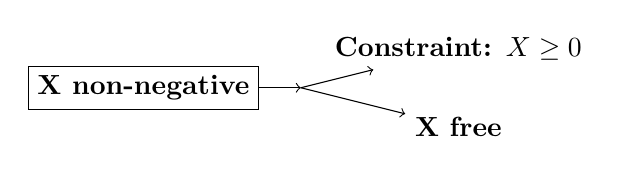
\begin{tikzpicture}[level distance=2cm, sibling distance=1cm,->,node distance=2cm, main node/.style={rectangle,draw,font=\bfseries}]

  \node[main node] (1) {X non-negative} 
  child[main node,grow=right] {
  child{node{X free}} child{node{Constraint: $X\geq 0$}}
  };
\end{tikzpicture}
\end{center}


\paragraph{Equalities and inequalities}
After treating the objective and the variables, it is important to treat the constraints (which offer the widest range of varieties). Firstly, turning equalities into inequalities is very straightforward:

\begin{center}
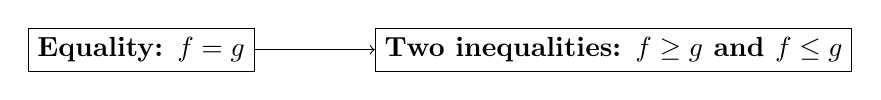
\begin{tikzpicture}[->,node distance=6cm, main node/.style={rectangle,draw,font=\bfseries}]

  \node[main node] (1) {Equality: $f = g$};
  \node[main node] (2) [right of=1] {Two inequalities: $f \geq g$ and $f \leq g$};

  \path[every node/.style={font=\sffamily\small}]
    (1) edge node [above] {} (2);
\end{tikzpicture}
\end{center}

The opposite is both more useful and more subtle:

\begin{center}
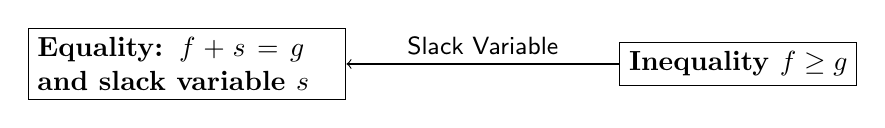
\begin{tikzpicture}[<-,node distance=7cm, main node/.style={rectangle,draw,font=\bfseries}]

  \node[main node,text width=3.8cm] (1) {Equality: $f + s = g $ and slack variable $s$};
  \node[main node] (2) [right of=1] {Inequality $f \geq g$};

  \path[every node/.style={font=\sffamily\small}]
    (1) edge node [above] {Slack Variable} (2);
\end{tikzpicture}
\end{center}

To do this, we must introduce the concept of \textbf{slack variable} (\textit{variable d'écart} in French). A slack variable is a non-negative variable added on the greater side of the inequality to make it an equality. Basically, its value is $f-g$, the slack between $f$ and $g$, representing the \textit{margin} before the constraint becomes an equality. 

One last case to be treated is the \textbf{lower bound constraint}. This can of course be treated as a constraint, but is redundant with the nonnegativity of the variables in the standard form. A fairly simple solution is to subtitute the variable $X$ with $X-l$, where $l$ is the lower bound.

\begin{center}
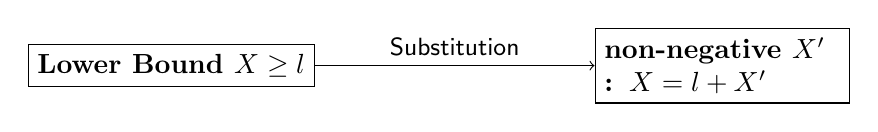
\begin{tikzpicture}[->,node distance=7cm, main node/.style={rectangle,draw,font=\bfseries}]

  \node[main node] (1) {Lower Bound $X \geq l$};
  \node[main node, text width=3cm] (2) [right of=1] {non-negative $X'$ : $X = l + X'$};

  \path[every node/.style={font=\sffamily\small}]
    (1) edge node [above] {Substitution} (2);
\end{tikzpicture}
\end{center}


\subsection{Standard form for linear models}
The standard form of a \textbf{linear optimization problem} is:
\begin{framed}
$$\begin{array}{cl}
\min_X & c^T X \\
 & A X = b \\
 & X \geq 0 \;\;\; (\Longleftrightarrow X \text{non-negative})
\end{array}$$
\end{framed}

If the problem has $n$ variables and $m$ constraints, then $c \in \mathbb{R}^{n\times 1}$, $A \in \mathbb{R}^{m\times n}$ and $b \in \mathbb{R}^{m\times 1}$. These constitute the only data needed to uniquely define the problem. 

The transformations exposed in the previous section illustrate the fact that it is possible to turn any linear optimization problem in the standard form.

\subsection{Standard form for convex models}
There is \textbf{no known standard form} for convex optimization problems. This can be understood in the sense that the objective function can be very general, as well as the set $X$. Since, by definition, the set $X$ is uncountable, it is very hard to represent it in a way that can be, for example, treated by a computer. However, it is possible, under certain assumptions, to represent the set $X$ in a purely functional way, as a set of inequalities involving functions.

Most often, the set $X$ is defined as a set of constraints. Let's suppose that there exists a set of functions $g_i$, $i \in \left\{1 \geq \dots \geq m \right\}$, $h_j$, $j \in \left\{ 1 \geq \dots \geq l \right\}$, such that:
$$X = \left\{ x \in \mathbb{R}^n | g_1(x) \leq 0, \dots, g_m(x) \leq 0 \text{ and } h_1(x)=0, \dots, h_l(x) = 0 \right\}$$

This form is general, since the $g_i(x) \geq 0$ constraint is equivalent to $-g_i(x) \leq 0$. The one exception lies in the fact that \textbf{strict inequalities} cannot be treated. But, as is explained later, this is not a real issue. 

In general, this does not suffice to guarantee that X is convex. The following conditions are \textbf{sufficient} to ensure the convexity of the set X:
\begin{itemize}
\item the $g_i$ functions are \textbf{convex} (this results from the choice that $g_i$ should be smaller than zero: if the opposite were chosen, then the functions should be concave)
\item the $h_j$ functions are \textbf{linear}: it's tempting to say that convexity is enough, but it is not the case. For example, the function $h:\mathbb{R}^2\rightarrow \mathbb{R}: (x,y) \rightarrow x^2+y^2 -1$ defined as ensemble $X$ the circle (and not the discus!) of radius 1, which is obviously not convex\footnote{In fact, each segment binding two points of the circle doesn't include any other point of the circle that its extremity\dots}.
\end{itemize}

In some cases, the constraints $h_j(x)=0$ can be relaxed to inequalities $h_j(x)=0$ \textcolor{red}{(Shouldn't it be an inequality?)}, thus relaxing the linearity constraint on $h_j$. One of these cases, which will be developed in the next section, is when the objective function is linear.


\begin{framed}\label{note_on_diff}
\textbf{A note on $\neq$} The standard forms developed in this section do not allow for strict inequalities to be considered. This is because strict inequalities tend to make solutions \textit{disappear}: in linear optimization, solutions are always located on the boundary of a closed polyhedron. By making this polyhedron open (with strict inequalities), the solutions disappear, as there is not admissible point with a minimal value (it is always possible to get \textit{closer} to the boundary, thus reducing the objective function).

A solution to this is to treat strict inequalities as non-strict ones by introducing a \textit{tolerance} $\epsilon > 0$, that describes how close to the open boundary the solutions can lie. The constraint $f>g$ then becomes $f \geq g+\epsilon$. The choice of the tolerance depends on the context of the problem (and is to be discussed with the client, for example).
\end{framed}

\subsection{Transforming \textit{any} problem into a convex problem}
We can turn any optimization problem into a convex problem by following two "easy" steps. First, \textit{the objective function can be made linear} by adding a new variable. Then, \textit{the constraints can be made convex} by an operation called taking the convex hull. Let us see these operations in detail.

\paragraph{First step : making the objective function linear}
Let us assume the following (general) model :

$$\min_{x \in X \subseteq \mathbb{R}^n} f(x)$$

The trick is to re-write this problem introducing a new variable $t$ that is greater or equal\footnote{It is intuitively more appealing to impose that $t = f(x)$, so we still have "exactly the same" objective function. But since equality constraints are harder to handle, we prefer the inequality $t \geq f(x)$. So instead of minimizing $f(x)$, we minimize \textit{a higher bound} to $f(x)$, wich is equivalent.} to $f(x)$.  We now have :

$$\min_{x \in \mathbb{R}^n, \; t \in \mathbb{R}} \: t \: \: \mathrm{with} \: \: x \in X, \: (x,t) \in epi \: f$$

The new objective function is just $t$ and is clearly linear, but the domain is now more complicated. In other words, we have traded simplicity in the objective function (wich is a good thing) by adding complexity in the domain (wich is usually already complex anyway, so it isn't that bad). Note that if the original problem was convex, the new problem is still convex (because it means $epi \: f$ is convex).

\paragraph{Second step : making the constraints convex}
The feasible set can be made convex by taking the convex hull of the set.\\

\begin{definition}
The \textbf{convex hull} of a set X (denoted by $conv \: X$) is the \textbf{smallest} convex set containing X. The smallest set means : the intersection of all possible convex sets containing X.
\end{definition}

\begin{example}
\begin{leftbar}
If we have a simple (non-convex) set containing two points in space, the convex hull of this set is the segment between those two points. This example is illustrated figure \ref{conv}. This gives us an (infeasible in practice, see "the catch" to make every problem convex, page \pageref{catch}) algorithm to take the convex hull of any set : just take every pair of points in the set and add the segment between those two points!

\end{leftbar}
\end{example}

\begin{figure}[h!]
\centering
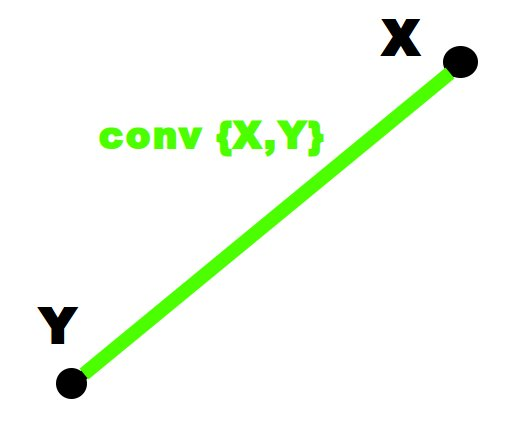
\includegraphics[scale=0.2]{./images/Course2_conv2}
\caption{Illustration of the convex hull of a set $X$. Note that the convex hull also includes the original set, wich is not very well represented on the figure.}
\label{conv}
\end{figure}

Taking the convex hull of the feasible set $X$ obviously gives us a new optimization problem. What are the optimal solutions of this new problem?\\

\begin{theorem}
Any optimal solution $x^*$ to the original problem :
$$\min_{x \in X} c^T x$$
is also optimal for the new problem :
$$\min_{x \in conv \: X} c^T x$$
\end{theorem}

This also means that the \textit{optimal values} of the two problems are the same. But because $X \subseteq conv \: X$, some optimal solutions of the new problem won't be in the original set $X$. So, in order to find the original optimal solutions, once we have solved the convex problem, we should always reject the optimal solutions of the new problems that aren't in $X$. Mathematically speaking : 
$$\{x^*_{original\,problem}\} = \{x^*_{new\,convex\,problem}\} \cap X $$

So, to summarize, we can make \textit{every problem in the world} convex, and we can (not yet, but after finishing this course) solve convex problems with good algorithms! This implies that basically any optimization problem can be solved easily! It seems too good to be true, and it is, since there is a \textbf{catch}\label{catch}. Although the definition of complex hull is rather simple, taking the convex hull of a general (that is, a little sophisticated) set is a very difficult operation.

So, in general, this approach is useless. There are specific cases, however, where this can be very useful!

The first, is a special case of linear optimization with \textbf{or} constraints. In such a problem, the admissible set is the union of (possibly disjoint) polyhedra. Computing the convex hull of the union of polyhedra can be done very efficiently, if the vertices are known, since the only task is to compute the vertices that will stay extreme in the union. The figure \ref{fig:my_label} illustrates this example.

\begin{figure}[H]
\centering
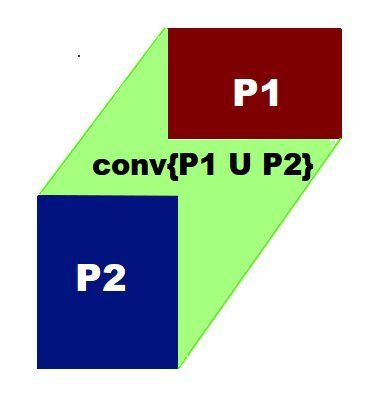
\includegraphics[scale=.4]{./images/Course2_polynoms}
\caption{Two (simple) disjoint polyhedron and the convex hull (in green) of the union.}
\label{fig:my_label}
\end{figure}

An interesting point to be raised here, is that such a problem could also be solved by computing the solution on every polyhedron, then choosing the best one. For small problems, this is of course valid, but for high number of dimensions, the cost of solving the problem on each polyhedron becomes prohibitive, while computing the convex hull remains a relatively cheap operation. 

The second case where taking the convex hull is useful is for (some) discrete models. Indeed:
$$\begin{array}{ccl}
\min_{x_i \in \{-1,1\}} c^T x & \Longleftrightarrow & min_{x} c^T x  \\
 & & -1 \leq x_i \leq 1
\end{array}$$

The convex hull of $\{-1,1\}^n$ is $[-1,1]^n$, and so both problems have the same solutions. The flow problem with integers (as seen in LINMA1702), which retains integer only solutions with relaxation, is an example of taking the convex hull of discrete problems without changing the nature of solutions. 

\subsection{Approximate \textit{any} convex problem by a linear problem}

It is possible to approximate convex problems by linear ones. Since the objective can always be converted to a linear function by adding a variable, the only work to be done concerns the constraints. Basically, the idea is to approximate the (closed\footnote{Why not open? Because an open set corresponds to strict inequalities, which cannot and will not be treated with the common optimization tools (see ``A note on $\neq$'', page \pageref{note_on_diff})}) set $X$ by a finite intersection of half-spaces (thus, linear constraints).

The way to do this is to use \textbf{projections} of points on the convex space. The projection of a point $u$ on a set $X$ is defined as the point $u_p \in X$ that minimizes the distance between itself and $u$.\\

\begin{theorem}{\textbf{Uniqueness and existence of projection.}}
Let $X$ be a \textbf{closed, non-empty, convex} set in $\mathbb{R}^n$, the projection of any exterior point on $X$ exists and is unique.
\end{theorem}

It is easy to see that the closeness and non-emptiness guarantee the existence of such projection. The unicity, however, is ensured by the convexity of the set. As an example, it is easy to see that a non-convex set such as the unit circle as an infinite number of projections of the origin.


With this concept of projection, we can introduce the \textbf{separation property}: for every exterior point $u$ of a convex closed set $X$, there exists a plane that \textit{separates} $u$ from $X$, that is, such that every element of $X$ is on \textit{one side} of the plane, while $u$ is on the \textit{other side}. This results directly from the uniqueness and existence of the projection of $u$ on $X$, although this was not demonstrated in class. Intuitively, this separation plane can be built perpendicular to the segment joining $u$ and its projection, without intersecting the convex plane.

So, to approximate a convex set by a linear one, the following method should be applied: for every point that should not be in $X$, create a separation plane. Such plane defines a half-space containing all of $X$. The intersection of all the half-spaces obtained this way forms a polyhedron containing $X$.

Moreover, it is interesting to note that an infinite number of points will create the convex set itself! This yields a new definition for a convex set: a convex set can always be written as the infinite intersection of half-spaces. This definition also proves immediately that every polyhedra is convex.

\begin{figure}[H]
\centering
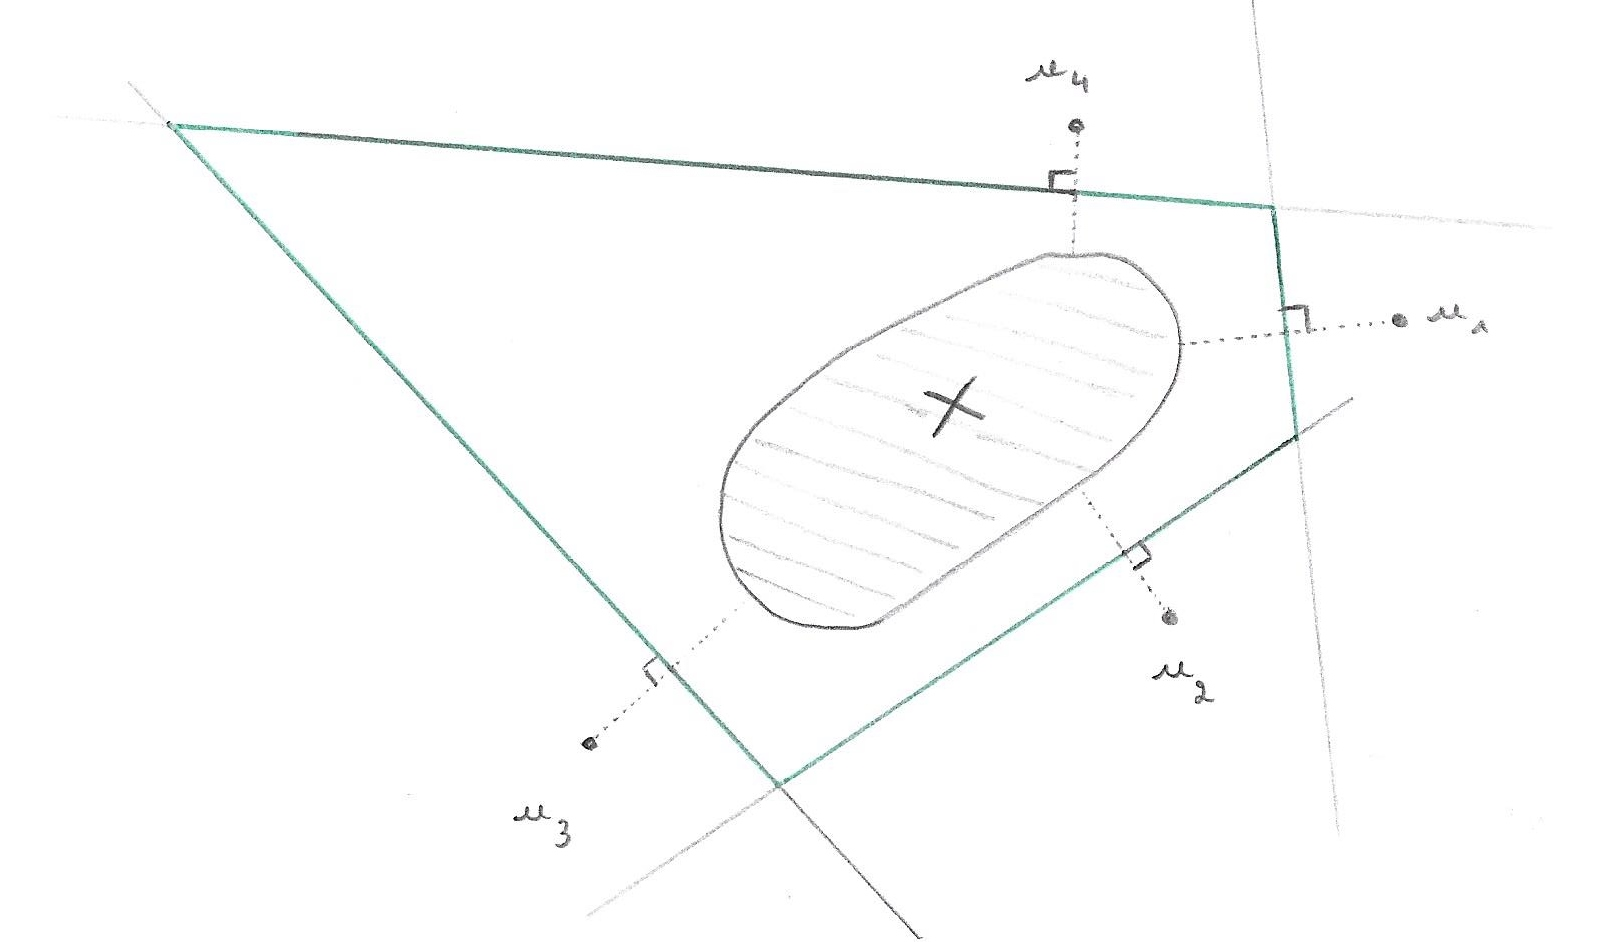
\includegraphics[scale=.4]{./images/Course2_Scan}
\caption{Approximation of a non-linear problem by a linear one.}
\label{labello}
\end{figure}
%\end{document}
